\documentclass[12pt, a4paper]{article}
\usepackage{graphicx} % Required for inserting images
\usepackage[paper=a4paper,top=1in,bottom=1in,right=1in,left=1in]{geometry}% http://ctan.org/pkg/geometry
\usepackage{amsmath, xparse}
\setcounter{MaxMatrixCols}{20}
\usepackage{caption}
\usepackage[framed, numbered]{matlab-prettifier}

\begin{document}

\begin{titlepage}
   \begin{center}
       
\includegraphics[width=0.25\textwidth]{img/metu.png}\\
       \vspace*{1cm}
       \Large
       \textbf{MIDDLE EAST TECHNICAL UNIVERSITY}\\
       \vspace{0.05cm}
       \textbf{DEPARTMENT OF MECHANICAL ENGINEERING}\\
       \vspace{1.2cm}
       \textbf{ME 310 – NUMERICAL METHODS}\\
       \textbf{SPRING 2022}\\
       \vspace{3cm}
       \text{HOMEWORK 2}\\
       \vspace{2cm}
       \text{Muhammed Rüstem ŞEVİK - 2446888}

       \vfill
       
       \small
       I understand that this is an individual assignment. I affirm that I have not given or received
any unauthorized help on this assignment, and that this work is my own.
            
       \vspace{0cm}

            
   \end{center}
\end{titlepage}

\newpage
    \renewcommand{\contentsname}{Table of Contents}
    \tableofcontents
\newpage

\section{Introduction}

This report aims to provide a solution to the given engineering problems using linear algebraic equation systems. The report addresses questions related to a truss structure, a steady one-dimensional heat conduction and a steady two-dimensional heat conduction problems, which require solving linear equation systems. For the truss problem, the report discusses three methods, MATLAB linsolve() function, naive Gaussian elimination and partial row pivoting Gaussian elimination to solve the system. For the heat conduction problems, the report presents Thomas algorithm, Cholesky decomposition and Gauss-Seidel algorithm. The report aims to provide a detailed analysis of the solutions obtained from each method and discuss the feasibility of the results.

\section{Body}
\subsection{Question 3}
The question asks for the solution of a given system by using various methods stated in separate parts. 
\begin{equation}
\begin{bmatrix}
0 & 0.9231 & 0 & 0 & 0 & 0 & 0 & 0 \\
1 & -0.3846 & 0 & 0 & 0 & 0 & 0 & 0 \\
0 & 0 & 0 & 0 & -1 & 0 & -0.8575 & 0 \\
-1 & 0 & -0.7809 & 0 & 0 & 0 & 0 & 0 \\
0 & 0.3846 & 0.7809 & 0 & 1 & -0.3846 & 0 & 0 \\
0 & -0.9231 & -0.6247 & 0 & 0 & 0.9231 & 0 & 0 \\
0 & 0 & 0.6247 & 1 & 0 & 0 & 0 & 0 \\
0 & 0 & 0 & -1 & 0 & 0 & 0.5145 & 1
\end{bmatrix} 
\begin{bmatrix}
F_{A B} \\
F_{A C} \\
F_{B C} \\
F_{B D} \\
F_{C D} \\
F_{C E} \\
F_{D E} \\
F_{D F} \\
\end{bmatrix}= 
\begin{bmatrix}
1690 \\
3625 \\
0 \\
0 \\
0 \\
0 \\
0 \\
0 \\
\end{bmatrix}
\end{equation}

\subsubsection{Part A}

The solution of the system by using linsolve function of MATLAB:

\begin{equation}
\begin{bmatrix}
F_{A B} \\
F_{A C} \\
F_{B C} \\
F_{B D} \\
F_{C D} \\
F_{C E} \\
F_{D E} \\
F_{D F} \\
\end{bmatrix}= 
\begin{bmatrix}
4329.1\\
1830.8\\
-5543.8\\
3463.2\\
2886.2\\
-1920.9\\
-3365.9\\
5194.9\\
\end{bmatrix}
\end{equation}
\subsubsection{Part B}
The solution of the system by using Naive.m code:

\begin{equation}
\begin{bmatrix}
F_{A B} \\
F_{A C} \\
F_{B C} \\
F_{B D} \\
F_{C D} \\
F_{C E} \\
F_{D E} \\
F_{D F} \\
\end{bmatrix}= 
\begin{bmatrix}
NaN\\
NaN\\
NaN\\
NaN\\
NaN\\
NaN\\
NaN\\
NaN\\
\end{bmatrix}\end{equation}
The solution is not the same as the part a.
Note that, $NaN$ (Not-a-Number) is a special value in MATLAB that represents undefined or unrepresentable numerical results. It can be returned in scenarios such as arithmetic operations involving undefined values, functions with undefined or unrepresentable results, or functions that encounter errors. $NaN$ can propagate through subsequent calculations, so it's important to handle $NaN$ values appropriately. The $isnan$ function can be used to check if a value is $NaN$.

\subsubsection{Part C}

Partial pivoting is a technique used in linear algebra when solving systems of equations. It involves swapping the rows of a matrix in order to ensure that the largest absolute value element of a column is placed in the pivot position. This helps to prevent numerical errors and instability when performing Gaussian elimination or LU decomposition. By using partial pivoting, the resulting solutions are more accurate and reliable.\\
The solution of the partial row pivoting Gaussian elimination code:
\begin{equation}
\begin{bmatrix}
F_{A B} \\
F_{A C} \\
F_{B C} \\
F_{B D} \\
F_{C D} \\
F_{C E} \\
F_{D E} \\
F_{D F} \\
\end{bmatrix}= 
\begin{bmatrix}
4329.1\\
1830.8\\
-5543.8\\
3463.2\\
2886.2\\
-1920.9\\
-3365.9\\
5194.9\\
\end{bmatrix}\end{equation}
The solution is the same as the part a. The reason of that the naive gaussian elimination is failed is that the division by zero case is not considered.
\subsubsection{Part D}
Highest tensile force member:
\begin{equation}F_{D F} = 5194.9\end{equation}
Highest compressive force member:
\begin{equation}F_{B C} = -5543.8\end{equation}
Considering the assumptions these results makes sense.

\subsubsection{Code}

\lstinputlisting[style=Matlab-editor, basicstyle=\mlttfamily\scriptsize]{Q3.m}



\newpage
\subsection{Question 4}
The question asks for the solution of the given system by using Thomas algorithm, Cholesky decomposition and iterative Gasuss-Seidel algorithm with relaxation.

\begin{equation}
\begin{bmatrix}
-2 & 1 &  &  &  &  &  \\
1 & -2 & 1 &  &  & &  \\
 & 1 & -2 & 1 &  &  &  \\
 &  & \cdot & \cdot & \cdot &  &  \\
 &  &  & \cdot & \cdot & \cdot &  \\
 &  &  &  & 1 & -2 & 1 \\
 &  &  &  &  & 1 & -2
\end{bmatrix}
\left\{\begin{array}{c}
T_{1} \\
T_{2} \\
T_{3} \\
\cdot \\
\cdot \\
\cdot \\
T_{N-1} \\
T_{N}
\end{array}\right\}=-\frac{\dot{q}(\Delta x)^{2}}{k}\left\{\begin{array}{l}
1 \\
1 \\
1 \\
\cdot \\
\cdot \\
1 \\
1
\end{array}\right\}+\left\{\begin{array}{c}
-T_{L} \\
0 \\
0 \\
\cdot \\
\cdot \\
\cdot \\
0 \\
-T_{R}
\end{array}\right\}
\end{equation}
\subsubsection{Part A}
The solution obtained by the Thomas algorithm as follows:
\begin{equation}
\left\{
\begin{array}{c}
T_{1} \\
T_{2} \\
T_{3} \\
T_{4} \\
T_{5} \\
T_{6} \\
T_{7} \\
T_{8} \\
T_{9} \\
T_{10} \\
T_{11} \\
T_{12} \\
T_{13} \\
T_{14} \\
T_{15}
\end{array}
\right\}=
\left\{
\begin{array}{c}
58.9844 \\
67.1875 \\
74.6094 \\
81.2500 \\
87.1094 \\
92.1875 \\
96.4844 \\
100.0000 \\
102.7344 \\
104.6875 \\
105.8594 \\
106.2500 \\
105.8594 \\
104.6875 \\
102.7344
\end{array}
\right\}
\end{equation}

\subsubsection{Part B}
The solution obtained by the Cholesky decomposition, forward and backward substitution the lower matrix $L$\\
Since the matrix is a banded matrix it is practical to write the matrix in two columns where for $D_{i} = L_{i,i}$ for $i = 1,..,15$ and $F_{i} = L_{i+1,i}$ for $i = 1,..,14 $

\begin{equation}
D =
\begin{bmatrix}
1.4142 \\
1.2247 \\
1.1547 \\
1.1180 \\
1.0954 \\
1.0801 \\
1.0690 \\
1.0607 \\
1.0541 \\
1.0488 \\
1.0445 \\
1.0408 \\
1.0377 \\
1.0351 \\
1.0328 \\
\end{bmatrix},
F =
\begin{bmatrix}
-0.7071 \\
-0.8165 \\
-0.8660 \\
-0.8944 \\
-0.9129 \\
-0.9258 \\
-0.9354 \\
-0.9428 \\
-0.9487 \\
-0.9535 \\
-0.9574 \\
-0.9608 \\
-0.9636 \\
-0.9661\\
\end{bmatrix}
\end{equation}
The solution obtained by the Cholesky decomposition, forward and backward substitution as follows:
\begin{equation}
\left\{
\begin{array}{c}
T_{1} \\
T_{2} \\
T_{3} \\
T_{4} \\
T_{5} \\
T_{6} \\
T_{7} \\
T_{8} \\
T_{9} \\
T_{10} \\
T_{11} \\
T_{12} \\
T_{13} \\
T_{14} \\
T_{15}
\end{array}
\right\}=
\left\{
\begin{array}{c}
58.9844 \\
67.1875 \\
74.6094 \\
81.2500 \\
87.1094 \\
92.1875 \\
96.4844 \\
100.0000 \\
102.7344 \\
104.6875 \\
105.8594 \\
106.2500 \\
105.8594 \\
104.6875 \\
102.7344
\end{array}
\right\}
\end{equation}
\noindent
The result is the same as the part a. This actively demonstrates that one may use a Cholesky decomposition to solve systems of linear equations.
\subsubsection{Part C}


Yes, the matrix with -2 on the main diagonal and 1 on the adjacent diagonals is diagonally dominant.

Diagonal dominance is a property of matrices where the absolute value of the diagonal elements is greater than or equal to the sum of the absolute values of the other elements in the same row. In this case, the absolute value of the diagonal element (-2) is greater than the sum of the absolute values of the other elements in the same row (which is equal to 1). This property ensures that the matrix is well-conditioned and invertible, and it can also help to ensure that certain numerical algorithms converge quickly and accurately.

Therefore, the matrix with -2 on the main diagonal and 1 on the adjacent diagonals is diagonally dominant.

\subsubsection{Part D}
The gauss seidel algorithm converged to the same solution with the given tolerance in 447 iterations.
\begin{equation}
\left\{
\begin{array}{c}
T_{1} \\
T_{2} \\
T_{3} \\
T_{4} \\
T_{5} \\
T_{6} \\
T_{7} \\
T_{8} \\
T_{9} \\
T_{10} \\
T_{11} \\
T_{12} \\
T_{13} \\
T_{14} \\
T_{15}
\end{array}
\right\}=
\left\{
\begin{array}{c}
58.9844 \\
67.1875 \\
74.6094 \\
81.2500 \\
87.1094 \\
92.1875 \\
96.4844 \\
100.0000 \\
102.7344 \\
104.6875 \\
105.8594 \\
106.2500 \\
105.8594 \\
104.6875 \\
102.7344
\end{array}
\right\}
\end{equation}

The relaxation parameter $\lambda$ affects convergence in Gauss-Seidel iteration by controlling the degree of relaxation between successive iterations. When $\lambda$ is closer to 1, the algorithm takes smaller steps towards the solution at each iteration, resulting in slower but more stable convergence. On the other hand, when $\lambda$ is further from 1, the algorithm takes larger steps towards the solution, resulting in faster but less stable convergence. The choice of $\lambda$ is therefore a trade-off between convergence speed and stability.

In the case of our problem, I observed that smaller $\lambda$ values lead to decrease in convergence rate and increasing $\lambda$ from 1 to 1.6 leads to faster convergence, as the number of iterations required to reach the desired tolerance decreases. This is because increasing $\lambda$ allows the algorithm to take larger steps towards the solution at each iteration, accelerating the convergence process.However, choosing $\lambda$ too large can lead to instability or divergence of the algorithm, as we have observed in our problem. Increasing $\lambda$ from 1.6 to 2 lead to slow down the convergence rate. Therefore, it is important to choose $\lambda$ carefully, balancing the desire for faster convergence with the need for stability and accuracy.

\begin{figure}
  \centering
  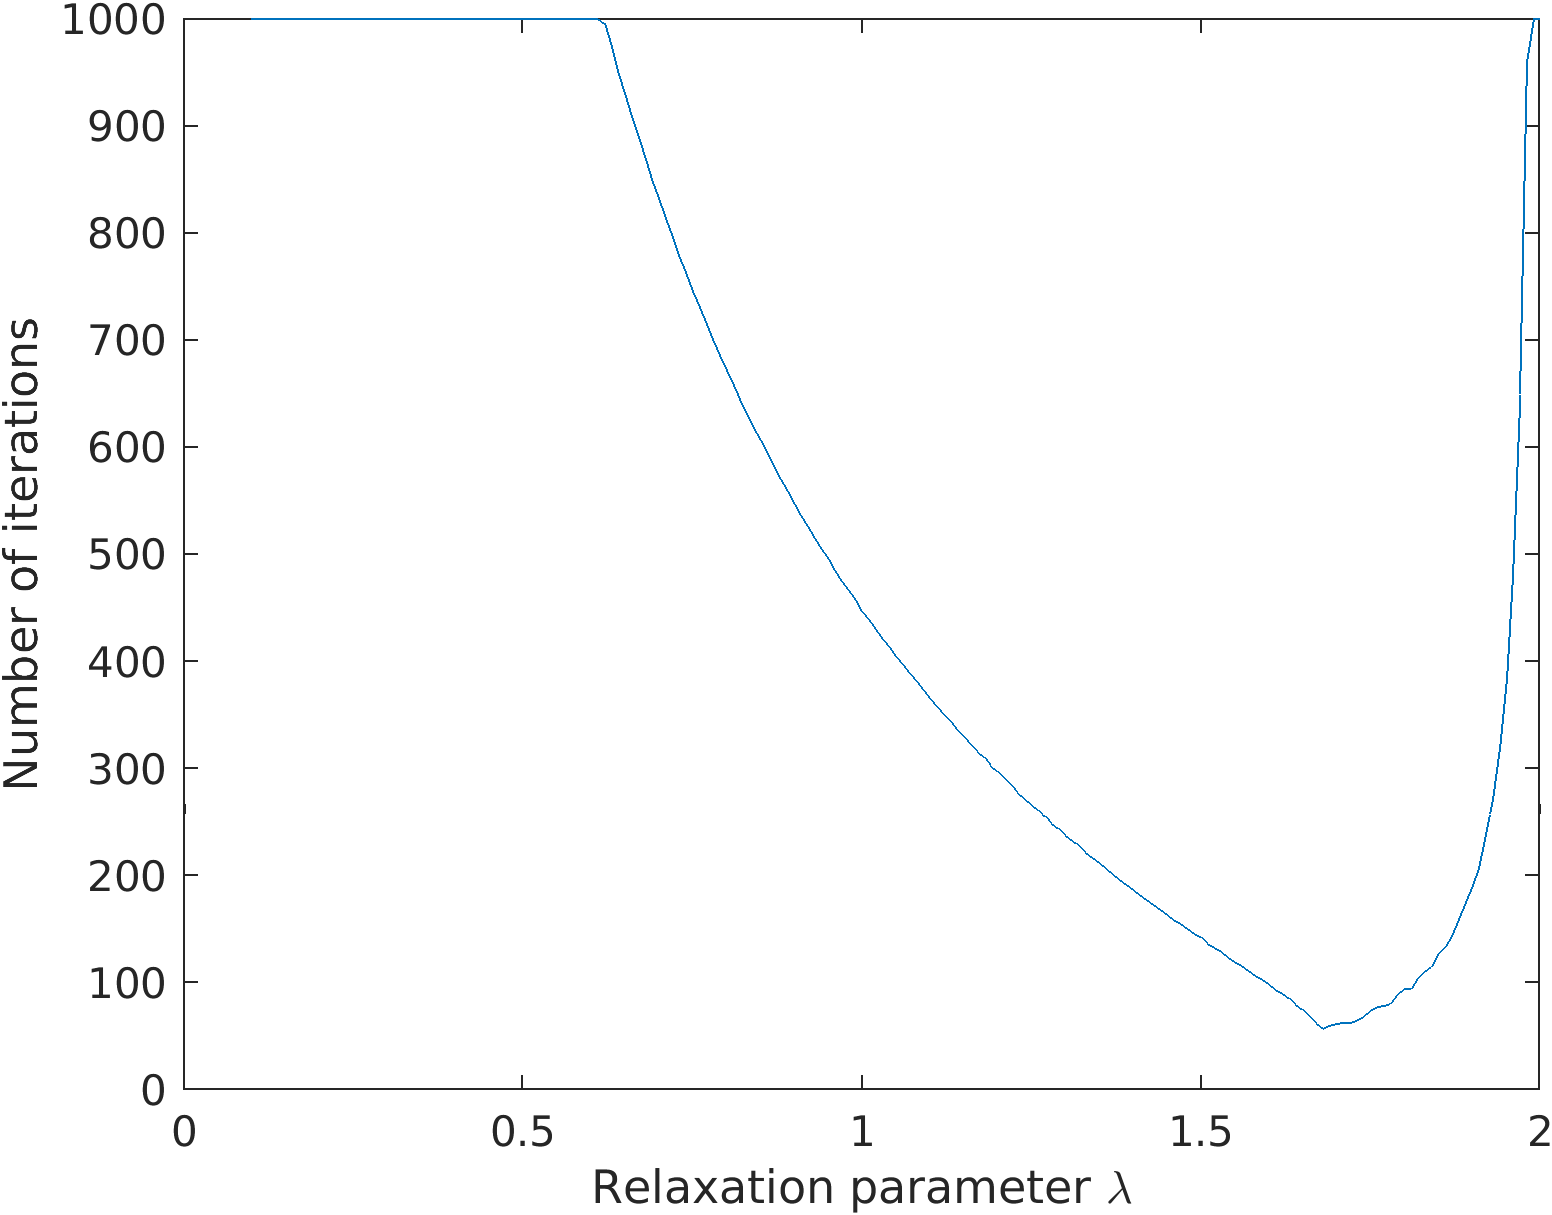
\includegraphics[width=0.9\textwidth]{img/lambda_vs_noi.png}
  \captionsetup{justification=centering}
  \caption{Relaxation Parameter $\lambda$ versus Number of Iterations}
\end{figure}

\newpage
\subsubsection{Code}
\lstinputlisting[style=Matlab-editor, basicstyle=\mlttfamily\scriptsize]{Q4.m}

\subsection{Question 5}
\subsubsection{Part A}
The temperature distribution inside the
plate is given by the following Laplace equation
\begin{equation}
\frac{\partial^2 T}{\partial x^2} + \frac{\partial^2 T}{\partial y^2} = 0
\end{equation}


To discretize the Laplace equation for any inner node $(i,j)$ use the following approximate derivatives:
\begin{equation}
\left.\frac{\partial^2 T}{\partial x^2}\right|_{i, j} \cong \frac{T_{i-1, j}-2 T_{i, j}+T_{i+1, j}}{(\Delta x)^2},\left.\quad \frac{\partial^2 T}{\partial y^2}\right|_{i, j} \cong \frac{T_{i, j-1}-2 T_{i, j}+T_{i, j+1}}{(\Delta y)^2}
\end{equation}
Plug the approximations into the Laplace equation
\begin{equation}
 \frac{T_{i-1, j}-2 T_{i, j}+T_{i+1, j}}{(\Delta x)^2} + \frac{T_{i, j-1}-2 T_{i, j}+T_{i, j+1}}{(\Delta y)^2} = 0
\end{equation}
For $\Delta x = \Delta y$ the equation simplifies to following form:
\begin{equation}
T_{i+1, j}+T_{i-1, j}+T_{i, j+1}+T_{i, j-1}-4 T_{i, j}=0
\end{equation}

To obtain the equations for $i=1,2,3$ and $j=1,2,3$, we substitute the corresponding values of $i$ and $j$ into the equation and simplify. 

\begin{equation}
    \begin{align}
        T_{2,1}+T_{0,1}+T_{1,2}+T_{1,0}-4T_{1,1}&=0\\
        T_{2,2}+T_{0,2}+T_{1,3}+T_{1,1}-4T_{1,2}&=0\\
        T_{2,3}+T_{0,3}+T_{1,4}+T_{1,2}-4T_{1,3}&=0\\
        T_{3,1}+T_{1,1}+T_{2,2}+T_{2,0}-4T_{2,1}&=0\\
        T_{3,2}+T_{1,2}+T_{2,3}+T_{2,1}-4T_{2,2}&=0\\
        T_{3,3}+T_{1,3}+T_{2,4}+T_{2,2}-4T_{2,3}&=0\\
        T_{4,1}+T_{2,1}+T_{3,2}+T_{3,0}-4T_{3,1}&=0\\
        T_{4,2}+T_{2,2}+T_{3,3}+T_{3,1}-4T_{3,2}&=0\\
        T_{4,3}+T_{2,3}+T_{3,4}+T_{3,2}-4T_{3,3}&=0\\
    \end{align}
\end{equation}

Construct the matrix A and vector b of the form $AT_{i,j} = b$:

\begin{equation}
\begin{bmatrix}
-4 & 1 & 0 & 1 & 0 & 0 & 0 & 0 & 0 \\
1 & -4 & 1 & 0 & 1 & 0 & 0 & 0 & 0 \\
0 & 1 & -4 & 0 & 0 & 1 & 0 & 0 & 0 \\
1 & 0 & 0 & -4 & 1 & 0 & 1 & 0 & 0 \\
0 & 1 & 0 & 1 & -4 & 1 & 0 & 1 & 0 \\
0 & 0 & 1 & 0 & 1 & -4 & 0 & 0 & 1 \\
0 & 0 & 0 & 1 & 0 & 0 & -4 & 1 & 0 \\
0 & 0 & 0 & 0 & 1 & 0 & 1 & -4 & 1 \\
0 & 0 & 0 & 0 & 0 & 1 & 0 & 1 & -4 \\
\end{bmatrix} 
\begin{bmatrix}
T_{1,1}\\
T_{1,2}\\
T_{1,3}\\
T_{2,1}\\
T_{2,2}\\
T_{2,3}\\
T_{3,1}\\
T_{3,2}\\
T_{3,3}\\
\end{bmatrix}=
\begin{bmatrix}
- T_{0,1} - T_{1,0}\\
- T_{0,2}\\
- T_{0,3} - T_{1,4}\\
- T_{2,0}\\  
0\\
- T_{2,4}\\ 
- T_{4,1} - T_{3,0}\\
- T_{4,2}\\
- T_{4,3} - T_{3,4}
\end{bmatrix}
\end{equation}


\subsubsection{Part B}

By using the linsolve function of the MATLAB the solution of the system as follows:
\begin{equation}
\begin{bmatrix}
T_{1,1}\\
T_{1,2}\\
T_{1,3}\\
T_{2,1}\\
T_{2,2}\\
T_{2,3}\\
T_{3,1}\\
T_{3,2}\\
T_{3,3}\\
\end{bmatrix}=
\begin{bmatrix}
57.8571\\
56.5625\\
47.1429\\
49.8661\\
46.2500\\
37.0089\\
45.3571\\
41.5625\\
34.6429\\
\end{bmatrix}
\end{equation}
The result makes sense because the distribution of the temperatures on the grid is as expected when the boundary temperatures are considered.
\subsubsection{Part C}
Yes there is an analytical solution of the Laplace equation.\\
The partial differential equation is:

\begin{equation}
\frac{\partial^2 T}{\partial x^2} + \frac{\partial^2 T}{\partial y^2} = 0
\end{equation}

Assuming the solution is separable, we write:

\begin{equation}
T(x,y) = X(x)Y(y)
\end{equation}

Substituting this into the Laplace equation and dividing by $X(x)Y(y)$, we get:

\begin{equation}
\frac{X''(x)}{X(x)} + \frac{Y''(y)}{Y(y)} = 0
\end{equation}

Since the left-hand side depends only on $x$ and $y$ separately, each side must be a constant, which we call $-\lambda^2$:

\begin{equation}
\frac{X''(x)}{X(x)} = \frac{Y''(y)}{Y(y)} = -\lambda^2
\end{equation}

This leads to two ordinary differential equations:

\begin{equation}
X''(x) + \lambda^2 X(x) = 0
\end{equation}

\begin{equation}
Y''(y) + \lambda^2 Y(y) = 0
\end{equation}

The general solutions to these equations are:

\begin{equation}
X(x) = A\cos(\lambda x) + B\sin(\lambda x)
\end{equation}

\begin{equation}
Y(y) = C\cos(\lambda y) + D\sin(\lambda y)
\end{equation}

where $A$, $B$, $C$, and $D$ are constants that depend on the boundary conditions.

The general solution to the Laplace equation is then:

\begin{equation}
T(x,y) = \sum_{n=1}^\infty \sum_{m=1}^\infty (A_{nm}\cos(\lambda_n x) + B_{nm}\sin(\lambda_n x))(C_{nm}\cos(\lambda_m y) + D_{nm}\sin(\lambda_m y))
\end{equation}

where $\lambda_n$ and $\lambda_m$ are the $n$th and $m$th positive roots of the equation $X''(x) + \lambda^2 X(x) = 0$, and $A_{nm}$, $B_{nm}$, $C_{nm}$, and $D_{nm}$ are constants determined by the boundary conditions.

\subsubsection{Code}
\lstinputlisting[style=Matlab-editor, basicstyle=\mlttfamily\scriptsize]{Q5.m}

\newpage
\section{Discussion}
The first question in this report is related to a truss problem with six joints and eight members. The task is to solve an 8x8 linear system using the linsolve function of MATLAB and the provided NaiveGE.m code. Additionally, the question requires implementing partial row pivoting to the NaiveGE.m code and solving the system again. Naive Gaussian elimination is failed due to division by zero case and in order to prevent it partial row pivotting is applied and the problem is solved.

The second question in this report involves solving a steady one-dimensional heat conduction problem using a tridiagonal system. The Thomas algorithm is applied to the tridiagonal system. The solution is obtained. Then Cholesky decomposition is applied and the solution is obtained. The solutions are the same. Then Gauss-Seidel algorithm is applied to the system again. In desired accuracy the solution is obtained in 447 iterations. The relaxation parameter is applied in the range of 0.1 to 2 and the results are plotted. The relaxation parameter effects positively when selected properly. If not it may cause the converging system to diverge. 

The third question is about the two-dimensional version of the previous problem. The question asks to construct the given system and solve it. The question also askes for the analytical solution of the system.

\section{Conclusion}

The homework is beneficial in terms of learning various analytical and iterative algorithms. I have also learned how these algorithms work and how parameters effect the accuracy of an algorithm. I have enhanced my ability to use MATLAB. This homework was very helpful to learn solution methods of systems of linear equations. Also in my case i have used latex to write the report. The report enhanced my ability to use tex environment.


\end{document}
